%% LLT: Turn off some annoying warnings...
\RequirePackage{silence}
\WarningFilter{titlesec}{Non standard sectioning command}
\WarningFilter{scrreprt}{Usage of package}
\WarningFilter{scrreprt}{Activating an ugly workaround}

% **************************************************
% Document Class Definition
% **************************************************
\documentclass[				%
	paper=A4,					% paper size --> A4 is default in Germany
%	twoside=true,				% onesite or twoside printing
    oneside=true,
%	twoside=false,				% onesite or twoside printing
	openright,					% doublepage cleaning ends up right side
	parskip=full,				% spacing value / method for paragraphs
	chapterprefix=true,			% prefix for chapter marks
	10pt,						% font size
	headings=normal,			% size of headings
	bibliography=totoc,			% include bib in toc
	listof=totoc,				% include listof entries in toc
	titlepage=on,				% own page for each title page
	captions=tableabove,		% display table captions above the float env
	draft=false, % value for draft version
]{scrreprt}						%

\usepackage{tocloft}
\usepackage{graphicx}				% Grafiken
\usepackage[utf8]{inputenc}			% defines file's character encoding
\usepackage{paralist}          		% for compactitem itemization
\usepackage{chngcntr}           		% Einfache Nummerierung von Abbildungen
\counterwithout{figure}{chapter} 	% Einfache Nummerierung von Abbildungen
\usepackage{listings} 				% Code Listings
\usepackage{float} 					% exaktes Figure Placement mit H
\usepackage{caption}          		% Figure-Captions formatieren
\lstset{
  breaklines=true,
%  numbers=left,
  numbersep=5pt,
  basicstyle=\footnotesize\ttfamily,
  numberstyle=\tiny\color{black}
%  literate=%
%  {Ö}{{\"O}}1
%  {Ä}{{\"A}}1
%  {Ü}{{\"U}}1
%  {ß}{{\ss}}2
%  {ü}{{\"u}}1
%  {ä}{{\"a}}1
%  {ö}{{\"o}}1
}
\lstset{literate=
  {á}{{\'a}}1 {é}{{\'e}}1 {í}{{\'i}}1 {ó}{{\'o}}1 {ú}{{\'u}}1
  {Á}{{\'A}}1 {É}{{\'E}}1 {Í}{{\'I}}1 {Ó}{{\'O}}1 {Ú}{{\'U}}1
  {à}{{\`a}}1 {è}{{\`e}}1 {ì}{{\`i}}1 {ò}{{\`o}}1 {ù}{{\`u}}1
  {À}{{\`A}}1 {È}{{\'E}}1 {Ì}{{\`I}}1 {Ò}{{\`O}}1 {Ù}{{\`U}}1
  {ä}{{\"a}}1 {ë}{{\"e}}1 {ï}{{\"i}}1 {ö}{{\"o}}1 {ü}{{\"u}}1
  {Ä}{{\"A}}1 {Ë}{{\"E}}1 {Ï}{{\"I}}1 {Ö}{{\"O}}1 {Ü}{{\"U}}1
  {â}{{\^a}}1 {ê}{{\^e}}1 {î}{{\^i}}1 {ô}{{\^o}}1 {û}{{\^u}}1
  {Â}{{\^A}}1 {Ê}{{\^E}}1 {Î}{{\^I}}1 {Ô}{{\^O}}1 {Û}{{\^U}}1
  {œ}{{\oe}}1 {Œ}{{\OE}}1 {æ}{{\ae}}1 {Æ}{{\AE}}1 {ß}{{\ss}}1
  {ű}{{\H{u}}}1 {Ű}{{\H{U}}}1 {ő}{{\H{o}}}1 {Ő}{{\H{O}}}1
  {ç}{{\c c}}1 {Ç}{{\c C}}1 {ø}{{\o}}1 {å}{{\r a}}1 {Å}{{\r A}}1
  {€}{{\EUR}}1 {£}{{\pounds}}1
}

\usepackage{minted} % needed for the inclusion of source code
\usepackage{textcomp}

% **************************************************
% Information and Commands for Reuse
% **************************************************
\newcommand{\thesisTitle}{Bachelorarbeit}
\newcommand{\thesisName}{Lukas Abegg}
\newcommand{\thesisMatrikelNr}{Matrikelnummer 798972}
\newcommand{\thesisSubtitle}{Suchoptimierung mittels maschinellen Lernens}
\newcommand{\thesisZeitraum}{Zeitraum 04.07.2016 - 04.10.2016}
\newcommand{\thesisSemester}{Sommersemester 2016}
\newcommand{\thesisDate}{Oktober 04, 2016}

\newcommand{\thesisFirstReviewer}{Prof. Dr. habil. Alexander Löser}
\newcommand{\thesisFirstPosition}{Fachbereich VI - Informatik und Medien}
\newcommand{\thesisFirstReviewerUniversity}{\protect{Beuth Hochschule f{\"u}r Technik}}
\newcommand{\thesisFirstReviewerUniversitySmall}{\protect{Beuth Hochschule}}
\newcommand{\thesisFirstReviewerUniversityCity}{Berlin}
\newcommand{\thesisFirstReviewerUniversityStreetAddress}{Luxemburger Str. 10}
\newcommand{\thesisFirstReviewerUniversityPostalCode}{13353}

\newcommand{\thesisSecondReviewer}{Prof. Dr. Martin Oellrich}
\newcommand{\thesisSecondPosition}{Fachbereich II - Mathematik - Physik - Chemie}
\newcommand{\thesisSecondReviewerUniversity}{\protect{Beuth Hochschule f{\"u}r Technik}}
\newcommand{\thesisSecondReviewerUniversitySmall}{\protect{Beuth Hochschule}}
\newcommand{\thesisSecondReviewerUniversityCity}{Berlin}
\newcommand{\thesisSecondReviewerUniversityStreetAddress}{Luxemburger Str. 10}
\newcommand{\thesisSecondReviewerUniversityPostalCode}{13353}

\newcommand{\thesisUniversity}{\protect{Beuth Hochschule f{\"u}r Technik}}
\newcommand{\thesisUniversityDepartment}{Studiengang Medieninformatik (B.Sc.)}
\newcommand{\thesisFachsemester}{Fachsemester 6}
\newcommand{\thesisUniversityCity}{Berlin}
\newcommand{\thesisUniversityStreetAddress}{Luxemburger Str. 10}
\newcommand{\thesisUniversityPostalCode}{13353}

% **************************************************
% Debug LaTeX Information
% **************************************************
%\listfiles

% **************************************************
% Load and Configure Packages
% **************************************************
\usepackage[german]{babel}    		% Deutsche Sprache in automatisch generiertem
\usepackage[							% use bachelorthesis style
	figuresep=colon,%
	sansserif=false,%
	hangfigurecaption=false,%
	hangsection=true,%
	hangsubsection=true,%
	colorize=full,%
	colortheme=bluemagenta,%
	bibsys=bibtex,%
	bibfile=bib-refs,%
	bibstyle=alphabetic,%
]{bachelorthesis}

\hypersetup{								% setup the hyperref-package options
	pdftitle={\thesisTitle},				% 	- title (PDF meta)
	pdfsubject={\thesisSubtitle},		% 	- subject (PDF meta)
	pdfauthor={\thesisName},				% 	- author (PDF meta)
	plainpages=false,					% 	-
	colorlinks=false,					% 	- colorize links?
	pdfborder={0 0 0},					% 	-
	breaklinks=true,						% 	- allow line break inside links
	bookmarksnumbered=true,				%
	bookmarksopen=true					%
}

\sloppy

% **************************************************
% Document CONTENT
% **************************************************
\begin{document}

% --------------------------
% rename document parts
% --------------------------
\renewcaptionname{german}{\figurename}{Abb.}
\renewcaptionname{german}{\tablename}{Tab.}
\renewcommand\listingscaption{Code}
\renewcommand\listoflistingscaption{Sourcecode-Verzeichnis}
\renewcaptionname{german}{\listfigurename}{Abbildungs-Verzeichnis}
\renewcaptionname{german}{\listtablename}{Tabellen-Verzeichnis}

% --------------------------
% Front matter
% --------------------------
\pagenumbering{roman}				% roman page numbing (invisible for empty page style)
\pagestyle{empty}					% no header or footers
% ------------------------------------  --> cover title page
\begin{titlepage}
	\pdfbookmark[0]{Cover}{Cover}
	\centering
	\hfill
	\vfill
	{\LARGE \color{ctcolortitle}\textbf{\thesisTitle} \\}
	\rule[2pt]{\textwidth}{.4pt} \\
	\Large{\thesisSubtitle} \\
	\small{\thesisZeitraum} \\[25mm]
	
	\begin{center}
	\Large\thesisName\\[5mm]
	\small{\thesisMatrikelNr} \\
	\small{\thesisSemester}\\
	\small{\thesisFachsemester}\\
	\small{\thesisUniversityDepartment} \\
	\small{\thesisUniversity}
	\end{center}		
	\par
	
	\vfill
	\begin{minipage}[t]{.35\textwidth}
		\raggedleft
		
\includegraphics[width=4.5cm]{gfx/beuth} \\[2mm]
	\end{minipage}
	\hspace*{15pt}
	\begin{minipage}[t]{.59\textwidth}
		{\Large \thesisFirstReviewerUniversity} \\
	  	{\small \thesisFirstReviewerUniversityStreetAddress} \\[-1mm]
	  	{\small \thesisFirstReviewerUniversityPostalCode\ \thesisFirstReviewerUniversityCity} 
	\end{minipage} \\[15mm]
	\begin{minipage}[t]{.35\textwidth}
		\raggedleft
		\textit{Betreuer}
	\end{minipage}
	\hspace*{15pt}
	\begin{minipage}[t]{.59\textwidth}
		\textbf{\thesisFirstReviewer} \\
		{\small \thesisFirstPosition\\
		\thesisFirstReviewerUniversity}
		\vskip 0.2in
	\end{minipage} \\[15mm]
	\begin{minipage}[t]{.35\textwidth}
		\raggedleft
		\textit{Gutachter}
	\end{minipage}
	\hspace*{10pt}
	\begin{minipage}[t]{.59\textwidth}
		\textbf{\thesisSecondReviewer} \\
		{\small \thesisSecondPosition\\
		\thesisSecondReviewerUniversity}
	\end{minipage} \\
\end{titlepage}
			% INCLUDE: all titlepages
\pagestyle{plain}					% display just page numbers

\setcounter{tocdepth}{3}				% define depth of toc
\tableofcontents						% display table of contents
\cleardoublepage

% --------------------------
% Body matter
% --------------------------
\pagenumbering{arabic}				% arabic page numbering
\setcounter{page}{1}					% set page counter
\pagestyle{maincontentstyle} 		% fancy header and footer

% !TEX root = ../Bachelorthesis.tex
%
%************************************************
% Einführung
%************************************************
\chapter{Einführung}
\label{sec:Einfuehrung}

Springer Nature ist ein weltweit führender Verlag für Forschungs-, Bildungs- und Fachliteratur mit einer breiten Palette an angesehenen und bekannten Medienmarken, zudem ist er der weltweit größte Verlag für Wissenschaftsbücher. Für das Unternehmen Springer Nature ist es darum wichtig auf seinen Web-Applikationen eine Suche anbieten zu können die Suchintentionen erkennt und möglichst schnell zum gesuchten Content leitet. Die Suche wird vor allem als Hilfsmittel zur Navigation und zum Finden von Literatur und Dienstleistungen genutzt. Durch die vielen von Springer Nature publizierten\footnote{Unter publizieren wird in dieser Arbeit die Veröffentlichung auf der Springermedizin-Applikation bezeichnet} Zeitschriften und Querverweise in Artikeln wird sie aber auch oft zur Suche nach Issues\footnote{Nummer der Zeitschriftenausgabe, in der sich der Artikel befindet} und Artikeln verwendet, sowie als Hilfestellung um Diagnosen zu Krankheitsbilder stellen zu können.
\\
\\
Springer Nature sammelt viele User-Tracking-Daten und dadurch viel Wissen über das Verhalten der User\footnote{Als User werden die Nutzer der Springer Nature Suche bezeichnet} bei der Nutzung ihrer Suche, lässt dieses Wissen jedoch bisher noch nicht in ihre Suche einfließen. In dieser Arbeit wollen wir untersuchen, ob mithilfe dieses Wissens, die Suche optimiert werden kann.

% Aufbau der Suche bei Springer Nature
%------------------------------------------------

\section{Aufbau der Suche bei Springer Nature}
\label{sec:Einfuehrung:AufbauSucheBeiSpringerNature}

\subsubsection{White Label Applikation mit Solr-Suche}
\label{sec:Einfuehrung:AufbauSucheBeiSpringerNature:WhiteLabelApplikationSolr-Suche}

Damit die verschiedenen Verlage und Zeitschriften der Verlagsgruppe Springer Nature ihre Produkte und Dienstleistungen online anbieten können, nutzt Springer Nature eine eigens entwickelte White Label Applikation\footnote{Eine White Label Applikation ist eine wiederverwendbare und agil erweiterbare Web-Applikation}. Die White Label Applikation verwendet \textit{Apache Solr}~(im Folgenden \glqq Solr\grqq{} genannt, siehe \cite{solr}) als Suchplattform. Die Solr dient hierbei als eine der Schnittstellen zwischen dem Content-Pool von Springer Nature und der White Label Applikation. Bei den vom Content-Pool gelieferten Inhalten handelt es sich um von Springer Nature Verlag publizierte Zeitschriften, Artikel, Bücher und redaktionelle Inhalte.

\subsubsection{User-Tracking mit Webtrekk}
\label{sec:Einfuehrung:AufbauSucheBeiSpringerNature:Webtrekk}

Um das Verhalten der User auf ihren Web-Applikationen zu tracken verwendet Springer Nature das Analysetool \textit{Webtrekk}~(siehe \cite{webtrekk}). Webtrekk wird als externer Webservice genutzt. Über diesen Webservice können die Tracking-Daten gelesen und ausgewertet werden. Die daraus resultierenden Berichte bieten unter anderem die Möglichkeit \textit{Suchquery-Logs}\footnote{Protokoll über alle ausgeführten Suchanfragen auf der Applikation} und \textit{Click-Through-Rates} (CTR)\footnote{Kennzahl um die Anzahl der Klicks auf Links im Verhältnis zu den gesamten Impressionen darzustellen} der User auszuwerten.

\pagebreak

\subsubsection{Architektur}
\label{sec:Einfuehrung:AufbauSucheBeiSpringerNature:Architektur}

In Abb. \ref{fig:SucheSpringerNature} ist die Suche nochmals grafisch aufbereitet:

\begin{figure}[H]
\centering
\vspace{-1.25em}
\caption[Aufbau der Suche bei Springer Nature]{Aufbau der Suche bei Springer Nature}
\vspace{.5em}
\label{fig:SucheSpringerNature}
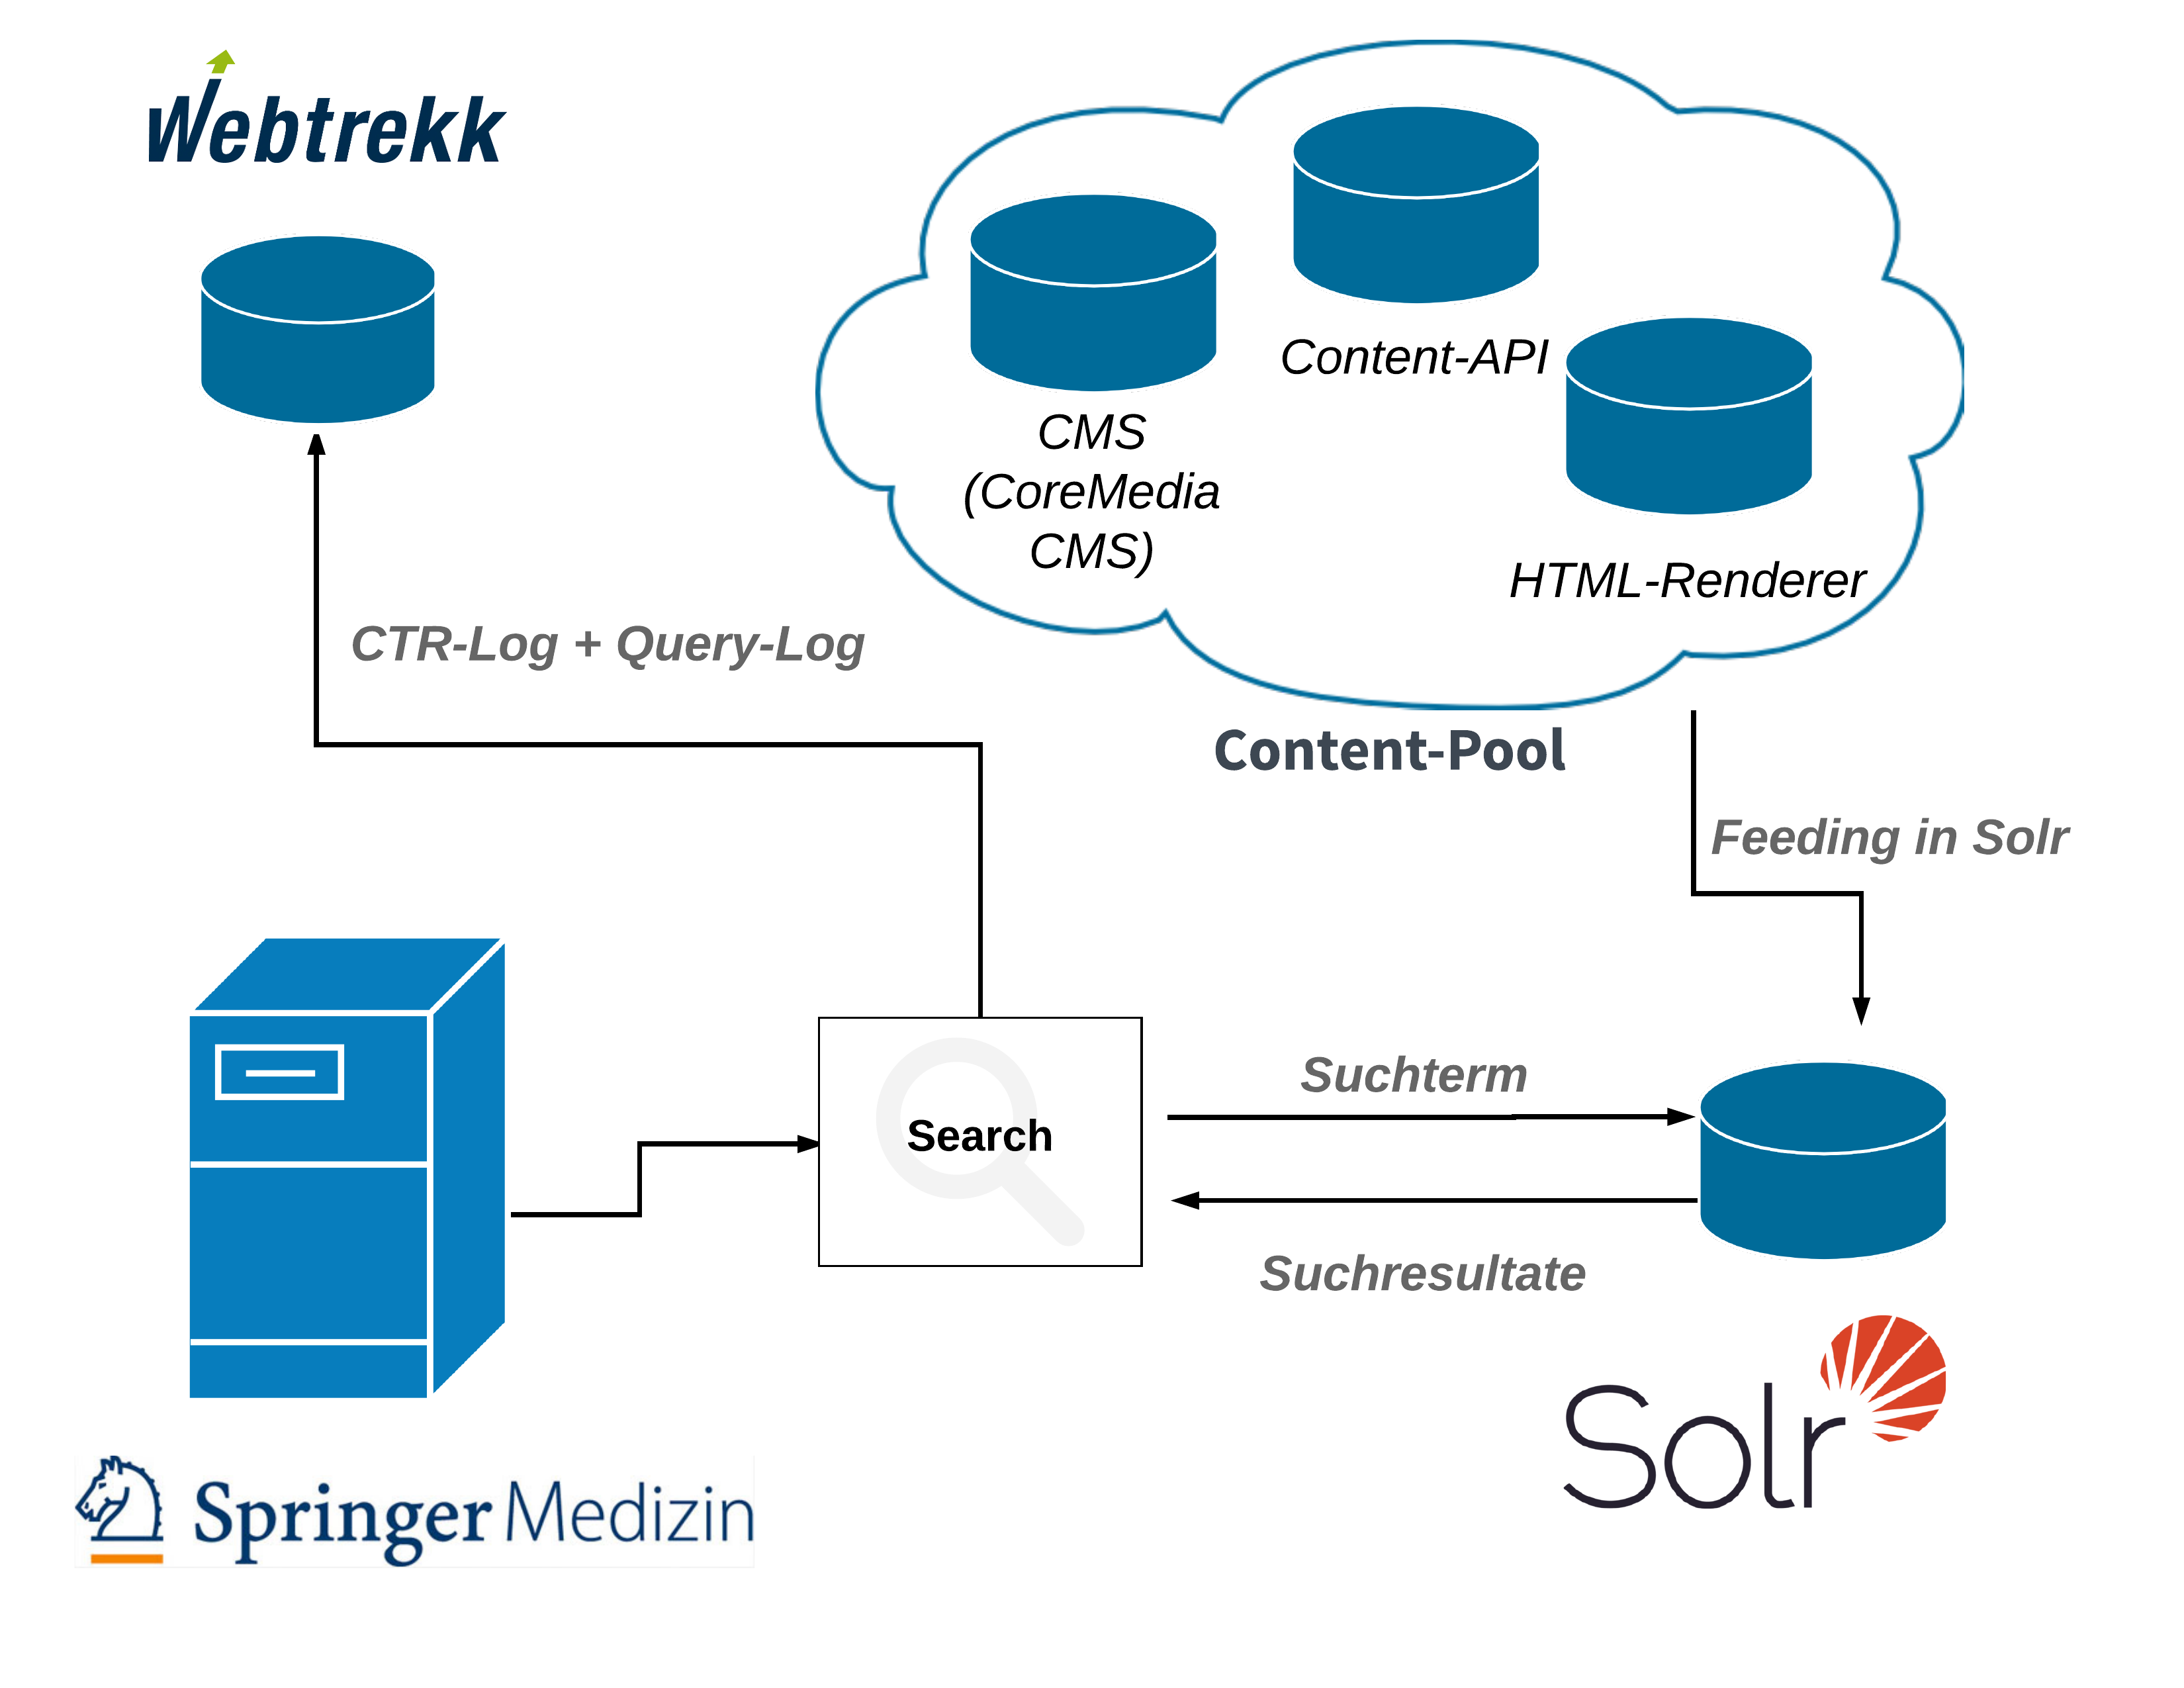
\includegraphics[width=0.7\linewidth]{gfx/AufbauSucheSpringerNature}
\vspace{-2em}
\end{figure}

% Problemstellung: Keine Userrelevanz in der Suche
%------------------------------------------------

\section{Problemstellung: Keine Userrelevanz in der Suche}
\label{sec:Einfuehrung:Problemstellung}

Zu den Stakeholder\footnote{Bezeichnet Springer Nature interne Kunden, die ein Interesse am Ergebnis der White Label Applikation haben}, der in Kapitel \ref{sec:Einfuehrung:AufbauSucheBeiSpringerNature:WhiteLabelApplikationSolr-Suche} angesprochenen White Label Applikation, gehört \textit{Springermedizin}~(siehe \cite{SMED}). Springermedizin betreibt ein Fortbildungs- und Informationsportal für Ärzte.

\subsubsection{Userrelevante Dokumente werden nicht gefunden}
\label{sec:Einfuehrung:Problemstellung:Userrelevanz}

Die User von Springermedizin suchen oft mit einschlägig, fundierten Fachbegriffen nach den neuesten und relevantesten Zeitschriften, Bücher oder Publikationen. Die zeitlich aktuellsten Suchtreffer zu finden ist für Springermedizin kein Problem. Die für den User \textit{relevantesten} jedoch schon.

\subsubsection{Der Springer Nature Stakeholder: Springermedizin setzt auf Webtrekk}
\label{sec:Einfuehrung:Problemstellung:Springermedizin}

Mithilfe von Webanalysten und Webtrekk versucht Springermedizin das Marketing seines Webauftrittes zu verbessern und ist sehr interessiert an neuen Ansätzen um die gesammelten Tracking-Daten besser einzusetzen. In dieser Arbeit wird darum der Fokus auf die Verwendung von Tracking-Daten in der Suche von Springermedizin gesetzt. 
 
\subsubsection{Der fast gläserne User}
\label{sec:Einfuehrung:Problemstellung:Glaeserne-User}

Springermedizin sammelt Tracking-Daten über jegliche Aktivitäten auf deren Applikationen und investiert Zeit und Geld in die Individualisierung\footnote{Mit Individualisierung wird die Speicherung eigener Parameter bezeichnet} der Analysedaten auf Webtrekk. Mittlerweile sind knapp 30 Custom-Parameter\footnote{Individuell erzeugte Parameter für Berichte und Analysen} auf Webtrekk angelegt, um genau die Daten zu tracken, die zur Analyse des Verhaltens der User auf ihrer Applikationen relevant sind. Dadurch entsteht ein fast \glqq gläsernen User\grqq{}. Dieses Wissen könnte zum Vorteil des Users eingesetzt werden indem es in der Suche verwendet wird.

\pagebreak
% Ziel der Arbeit
%------------------------------------------------
\section{Ziel der Arbeit}
\label{sec:Einfuehrung:ZielArbeit}

\subsection{Suchoptimierung durch Click-Through-Daten}
\label{sec:Einfuehrung:ZielArbeit:Suchoptimierung}

In dieser Arbeit werden wir untersuchen ob mithilfe der von Springermedizin gesammelten Click-Through-Daten\footnote{Mit Click-Through-Daten bezeichnen wir alle Tracking-Daten, welche während der Interaktion zwischen User und Suche protokolliert werden} deren Suche verbessert werden kann. Konkret wollen wir dies anhand eines Algorithmus basierend auf dem Klick-Modell\footnote{Als Klick-Modell wird ein Modell zur Berechnung des Userfeedbacks bzw. der Userrelevanz mithilfe von Click-Through-Daten bezeichnet} \textit{Position-Based Modell}~(PBM, siehe \cite{pbm}) untersuchen.

\subsubsection{Annahmen}
\label{sec:Einfuehrung:ZielArbeit:Suchoptimierung:Annahmen}

Wir gehen dabei von zwei Annahmen aus. Zum einen dass relevante Dokumente wichtiger sind, als nicht relevante Dokumente und zum anderen dass ein Suchergebnis dann gut ist, wenn die relevanten Ergebnisse in der verwendeten Hierarchie vor den nicht relevanten Ergebnissen auftauchen. 

\subsubsection{Anwendung auf das Springermedizin-Umfeld}
\label{sec:Einfuehrung:ZielArbeit:Suchoptimierung:AnwendungSpringermedizin-Umfeld}

Wir werden versuchen die CTRs der Suchresultate, mithilfe des oben angesprochenen Algorithmus, zu berechnen und mit diesen ein \textit{Reranking}\footnote{Mit Reranking bezeichnen wie die Umsortierung einer Liste von Suchresultaten} der Suchresultate auf das Springermedizin-Umfeld abzubilden. Die Herausforderung wird hierbei die Adaptierung des Lösungsansatzes auf das Springermedizin-Umfeld sein. Im Idealfall werden die gesammelten Click-Through-Daten die Userrelevanz der einzelnen Dokumente\footnote{Als Dokumente werden die einzelnen Suchresultate bezeichnet} widerspiegeln.

\subsection{Abbildung auf das Springermedizin-Umfeld}
\label{sec:Einfuehrung:ZielArbeit:AbbildungSpringermedizinUmfeld}

\subsubsection{Potential von Userrelevanzen in der Suchoptimierung analysieren}
\label{sec:Einfuehrung:ZielArbeit:Potential}

Die Analyse von User-Tracking-Daten bietet viel Potential bezogen auf Userrelevanzen. Falls anhand des hier umgesetzten Lösungsansatzes Verbesserungen in der Qualität der Suche zu verzeichnen sind, möchte Springermedizin in Zukunft vermehrt User-Tracking-Daten in die Suche einfließen lassen. Diese Arbeit könnte dann als Fundament für weitere Lösungsansätze dienen.

\subsubsection{Bekanntes und wirkungsvolles Information Retrieval Verfahren}
\label{sec:Einfuehrung:ZielArbeit:AbbildungSpringermedizinUmfeld:InformationRetrievalVerfahren}

Suchoptimierung mittels Userrelevanz ist ein bekanntes und nicht triviales, aber relativ wirkungsvolles Information Retrieval Verfahren~(siehe \cite{IWUSBI}). Seit Mitte der 2000er Jahre wird mithilfe dieses Verfahrens versucht Suchmaschinen zu verbessern. Aus dieser Zeit stammen auch die ersten Ansätze, um mithilfe von Click-Through-Daten die Userrelevanz der Suchergebnisse zu berechnen~(siehe \cite{Joachims}).

\subsubsection{Lösungsansatz basierend auf Click-Through-Daten aus Webtrekk}
\label{sec:Einfuehrung:ZielArbeit:AbbildungSpringermedizinUmfeld:Loesungsansatz}

Springermedizin führt ein eigenes Tracking der User durch und verwendet auf Webtrekk selbst definierte Tracking-Parameter. Dadurch hängt die Wahl des in dieser Arbeit zu untersuchenden Lösungsansatzes und dessen Umsetzung stark von den durch Webtrekk gegebenen Analyse-Daten ab.

\subsubsection{Keine Gegenüberstellung mit anderen Lösungsansätzen}
\label{sec:Einfuehrung:ZielArbeit:AbbildungSpringermedizinUmfeld:NichtBehandeln}

Bedingt durch den vorgegebenen Zeitraum für die Erstellung dieser Bachelorarbeit, werden wir den Lösungsansatz so wählen, dass er mit den Gegebenheiten bei Springermedizin sinnvoll und in diesem Zeitrahmen realistisch implementiert werden kann. Wir werden daher in dieser Arbeit keine Gegenüberstellung mit anderen Lösungsansätzen machen. 

% Methodik
%------------------------------------------------

\section{Methodik}
\label{sec:Einfuehrung:Methodik}

Wie in Kapitel \ref{sec:Einfuehrung:ZielArbeit:Suchoptimierung} angesprochen wollen wir das Klick-Verhalten der User in der Suche analysieren um mithilfe der daraus berechenbaren CTRs, die Suchergebnisse zu verbessern. Dieses Klick-Verhalten können wir aus den Click-Through-Daten lesen. 

\subsubsection{Suchterm semantisch aufschlüsseln}
\label{sec:Einfuehrung:Methodik:SuchtermSegmentierung}

Um mit den Click-Through-Daten arbeiten zu können, müssen wir zunächst die relevanten Click-Through-Daten herausfiltern. Dazu müssen wir die Click-Through-Daten dem \textit{Suchterm}\footnote{Als Suchterm wird die Sammlung aller, in der Suchanfrage verwendeten Wörter bezeichnet} der Anfrage zuordnen können. Zu den Click-Through-Daten wird immer der Suchterm gespeichert mit dem dabei gesucht wurde. Das heißt wir können eine Relation zwischen dem Suchterm der Click-Through-Daten und dem Suchterm unserer Anfrage herstellen.
\\
\\
Die Click-Through-Daten müssen aber nicht mit dem vollständigen Suchterm in Relation stehen. Sie können auch nur mit einem Wort, einem Teil des Suchterms oder einem Synonym eines dieser Worte in Relation stehen. Wir müssen darum den Suchterm semantisch aufschlüsseln, um alle relevanten Click-Through-Daten filtern zu können. 

\subsubsection{Aufbereitung Click-Through-Daten}
\label{sec:Einfuehrung:Methodik:Click-Through-Daten}

Können wir alle relevanten Click-Through-Daten zu einer Suchanfrage filtern, müssen wir lernen diese richtig aufzubereiten um die CTR berechnen zu können.  Ein wichtiger Punkt bei der Aufbereitung der Click-Through-Daten ist die Interpretation des Relevanzfeedbacks der einzelnen Click-Through-Daten. Nicht jeder Klick ist gleich relevant zu interpretieren. Die Relevanz eines Klicks hängt davon ab, welche Aktionen der User während dem Suchvorgang \textit{vor} und \textit{nach} dem Klick durchgeführt hat. Wir müssen darum zuerst analysieren, welche Informationen wir zu den Click-Through-Daten aus Webtrekk lesen können.  Reichen diese Informationen für detailliertere Interpretationen nicht aus, müssen wir alle Click-Through-Daten als gleich relevant lesen.

\subsubsection{Result-Reranking mittels PBM basierten Algorithmus}
\label{sec:Einfuehrung:Methodik:Result-RerankingPBM}

Sobald wir wissen wie man die Click-Through-Daten aufbereitet, können wir diese zur Berechnung der CTR eines Dokumentes, und somit dessen Userrelevanz, einsetzen. Für die Verwendung dieser Userrelevanz müssen wir festlegen, wann und in welcher Art wir sie einsetzen. Wie bereits in Kapitel \ref{sec:Einfuehrung:ZielArbeit:Suchoptimierung:AnwendungSpringermedizin-Umfeld} erwähnt, werden wir uns in dieser Arbeit auf die \textit{Aufbereitung} der Suchresultate aus der Solr konzentrieren und dort einen \textit{Reranking-Algorithmus} einbauen. 
\\
\\
Der Reranking-Algorithmus basiert auf dem \textit{Klick-Modell PBM}. Ein Klick-Modell verwendet die Click-Through-Daten, um daraus die CTR eines Dokumentes zu berechnen. Die Wahl des Klick-Modells hängt darum stark von den Click-Through-Daten und den darin enthaltenen Informationen ab. Das PBM setzt sich aus zwei Wahrscheinlichkeiten zusammen. Die Wahrscheinlichkeit für einen Klick auf die Position im Suchresultat und die Wahrscheinlichkeit für einen Klick auf das Dokument. In dieser Arbeit werden wir veranschaulichen, warum wir den Ansatz des PBMs~(siehe \cite{pbm}) gewählt haben und wie wir den Algorithmus umgesetzt haben.

\subsubsection{Vergessen der alten Daten}
\label{sec:Einfuehrung:Vergessen}

Das PBM berechnet Wahrscheinlichkeiten, um die CTR eines Dokumentes zu einer Suchanfrage festzustellen. Dem Algorithmus muss dazu das notwendige Wissen entweder zur Verfügung gestellt oder antrainiert werden. Wird dem Algorithmus das Wissen antrainiert, benötigt der Algorithmus eine Möglichkeit neues Wissen zu Lernen und Altes zu vergessen. 
\\
\\
Mit Webtrekk haben wir eine Wissensbasis, die durch die Springermedizin-Applikation automatisch um neue Click-Through-Daten ergänzt wird. Das heißt wir müssen uns nicht um eine Möglichkeit zum Lernen neuer Daten kümmern. Wir müssen uns aber überlegen, wie wir altes Wissen vergessen und wie wir dem User neues Wissen präsentieren, damit dieser sich durch die CTR-Berechnung nicht auf alten Dokumenten festfährt.

% Gliederung und Aufbau
%------------------------------------------------

\section{Gliederung und Aufbau}
\label{sec:Einfuehrung:GliederungAufbau}

\subsubsection{Der Lösungsansatz und deren Grundlagen}
\label{sec:Einfuehrung:GliederungAufbau:Loesungsansatz}

In diesem Kapitel wurde der zu untersuchende Lösungsansatz vorgestellt. Wir haben Problemstellungen und deren Teilprobleme identifiziert. Dabei sind wir auf die Hintergründe dieser Arbeit und die Vorgehensweise eingegangen. Im zweiten Kapitel~(Grundlagen) folgt die Theorie des beschriebenen Lösungsansatzes. Hier werden wir uns auf die fachlichen Grundlagen konzentrieren, Problemstellungen analysieren und Lösungsansätze vorstellen.

\subsubsection{Umsetzung des Lösungsansatzes}
\label{sec:Einfuehrung:GliederungAufbau:Umsetzung}

In Kapitel \ref{sec:Reranking}~(Reranking mittels CTR) werden wir die in Kapitel \ref{sec:Einfuehrung:Methodik} angesprochene Methodik verfeinern und auf Basis der Grundlagen aus Kapitel \ref{sec:Grundlagen:Grundbegriffe}, über die detaillierte Vorgehensweise bei der Umsetzung diskutieren. Die Umsetzung selbst folgt dann in Kapitel \ref{sec:Implementierung}~(Implementierung).

\subsubsection{Erkenntnisse verarbeiten}
\label{sec:Einfuehrung:GliederungAufbau:Erkenntnisse}

Um zu prüfen ob der umgesetzte Lösungsansatz die erhofften Verbesserungen erzielt, werden wir diesen in Kapitel \ref{sec:Evaluation}~(Evaluation und Auswertung) in einer Evaluation mit der bisherigen Springermedizin-Suche vergleichen. Aufgrund der resultierenden Erkenntnisse, werden wir in Kapitel \ref{sec:ZusammenfassungAusblick}~(Zusammenfassung und Ausblick) ein Fazit ziehen können und einen Ausblick auf mögliche, zukünftige Arbeiten geben. 	% INCLUDE: Einführung
% !TEX root = ../thesis-example.tex
%
%************************************************
% Grundlagen
%************************************************
\chapter{Grundlagen}
\label{sec:Grundlagen}

% Grundbegriffe
%************************************************

\section{Grundbegriffe}
\label{sec:Grundlagen:Grundbegriffe}

In diesem Kapitel werden wir die fachlichen Grundlagen zu unserem in Kapitel \ref{sec:Einfuehrung:Methodik} vorgestellten Lösungsansatz aufarbeiten. Wichtig hierfür ist das Verständnis für die Problemstellungen in der Interaktion zwischen den Nutzern der Suche und der Suche selbst und warum unser verfolgter Lösungsansatz schief gehen kann. Dazu gehört die Auseinandersetzung mit dem Klick-Verhalten der User auf der Suche von Springermedizin. Mit der Click-Trough-Rate wollen wir eine Userrelevanz bestimmen. Dazu müssen wir die Click-Trough-Daten als Relevanz-Feedback deuten können. Wie wir die Click-Trough-Rates berechnen, lernen wir in den Grundlagen zu unserem Reranking-Algorithmus. Diese Grundlagen sind notwendig für die Umsetzung des Lösungsansatzes in den nachfolgenden Kapiteln \ref{sec:Reranking} und \ref{sec:Implementierung}. In diesem Kapitel und dem darauf folgenden, werden Formeln mit selbst definierten Symbolen eingeführt. Folgend eine Legende zu den wichtigsten Symbolen:

\begin{table}[H]
\centering
\vspace{-.5em}
\caption[Legende der wichtigsten Formel-Symbolen für diese Arbeit]{Legende der wichtigsten Formel-Symbolen für diese Arbeit}
\label{tab:LegendeSymboleFormeln}
\vspace{-.5em}
\footnotesize
\renewcommand*{\arraystretch}{1.2}
\begin{tabular}{clcl} \hline
\textbf{Symbol} & \textbf{Bedeutung} & \textbf{Symbol} & \textbf{Bedeutung} \\ \hline
$u$	& ein Dokument im Suchergebnis & $C$	& das Dokument wird vom User \\ &&& im Suchergebnis angeklickt \\ 
$q$	& ein Suchterm & $E_{u}$	& das Dokument wird aufgrund seiner Position \\ &&& im Suchergebnis angeschaut \\
$r$	& die Position des Dokumentes im Suchergebnis &  $A_{u}$	& das Dokument wird aufgrund seines Suchsnippets \\ &&& im Suchergebnis angeschaut \\ 
$c$	& ein Klick auf ein Dokument im Suchergebnis & $X_{u}$	& ein Zufallswert der einem Dokument \\ &&& des Suchergebnisses zugewiesen wird \\
$s$ 	& eine Suchanfrage & $r_{X_{u}}$	& $r$ in der nach Zufallsfaktor \\ &&& sortierten Liste der Suchergebnisse \\ 
$S$	& eine Set von Suchanfragen & $r_{P(C_{u})}$ 	& $r$ in der nach Klick-Wahrscheinlichkeit \\ &&& sortierten Liste der Suchergebnisse \\
$P$	& die Wahrscheinlichkeit dass ein Fall eintritt &  $R_{u}$	& durch den Reranking-Algorithmus berechneter \\ &&& Relevanz-Wert des Dokumentes $u$ \\
\hline
\end{tabular}
\vspace{-2em}
\end{table}

% Semantik von User-Interaktionen
%------------------------------------------------

\subsection{Semantik von User-Interaktionen}
\label{sec:Grundlagen:Grundbegriffe:SemantikUserInteraktionen}

\subsubsection{Problemstellungen der Click-Trough-Daten: Was analysieren wir?}
\label{sec:Grundlagen:Grundbegriffe:SemantikUserInteraktionen:ProblemstellungenClick-Trough-Daten}

\paragraph{Einzelne Wörter oder Teile des Suchterms können in weiteren Suchanfragen vorkommen}
Ein Suchterm kann aus einem oder mehreren Wörtern bestehen. Jeder User formuliert eine Suchanfrage anders. Sei es die Wortwahl, die Zeitform oder die Verwendung von Bindewörtern. Daraus lässt sich vermuten, dass einzelne Wörter oder Teile des Suchterms in weiteren Suchanfragen vorkommen können. Folglich muss der Suchterm semantisch aufgeschlüsselt werden, um Relationen zwischen Click-Trough-Daten und der Suchanfrage herstellen zu können. Nur so können wir alle relevanten Click-Trough-Daten filtern.

\paragraph{Suchanfragen mit Synonymen und verwandten Begriffen beachten}
Nehmen wir als Beispiel die Suchanfrage \glqq chronische Dyspnoe\grqq{}. Würden wir stattdessen den sinnverwandten Suchterm \glqq konstante Atemnot\grqq{} verwenden, würden wir für beide Fälle ähnliche Suchresultate erwarten. Folglich würden wir auch ähnliche Click-Trough-Daten vermuten. Wir sollten daher die Synonyme und verwandte Begriffe zu unserem Suchterm ebenfalls beachten und deren Click-Trough-Daten, in den Reranking-Algorithmus einfließen lassen. Dazu benötigen wir eine Wissensbasis, welche die Synonyme und verwandte Begriffe zu unserem Suchterm gespeichert hat. Eine solche Basis bieten Wörterbücher und Thesauri\footnote{Thesauri sind strukturierte Verzeichnisse von Begriffen, die allesamt in irgendeiner Beziehung zueinander stehen bezeichnet}. Beim Content von Springermedizin handelt es sich um medizinische Inhalte in deutscher Sprache. Es macht daher Sinn dies in der Wahl der richtigen Wissensbasis zu berücksichtigen.

\subsubsection{Problemstellungen des Lösungsansatzes: Warum kann es schief gehen?}
\label{sec:Grundlagen:Grundbegriffe:SemantikUserInteraktionen:ProblemstellungenLoesungsansatz} 

Die folgenden Faktoren leiten sich aus dem verfolgten Lösungsansatz des Reranking-Algorithmus ab, bzw. werden in diesem nicht beachtet. Wir müssen davon ausgehen dass diese das Untersuchungsergebnis des Lösungsansatzes negativ beeinflussen könnten.

\paragraph{Die Relation des Suchterms zu den Click-Trough-Daten wird nicht gewichtet}
Die Click-Trough-Daten sind dann relevant, wenn mindestens ein Wort des aufgeschlüsselten Suchterms in Relation zu diesen Daten steht. Dadurch können falsche Relationen entstehen und nicht relevante Click-Trough-Daten die Klick-Wahrscheinlichkeiten der Dokumente im Reranking-Algorithmus negativ beeinflussen.

\paragraph{Intentionen und die Mehrdeutigkeit von Suchbegriffen werden nicht beachtet}
Die genaue semantische Analyse eines Suchterms beinhaltet unter anderem die Erkennung von Begriffen und deren Mehrdeutigkeiten. Suchte jemand z.B. nach dem Begriff \glqq Brücke\grqq{}, hat dieser im medizinischen Kontext mehrere Bedeutungen. Es könnte ein \glqq ein Teil des zentralen Nervensystems\grqq{} gemeint sein oder eine \glqq Form des Zahnersatzes\grqq{}. Wie bereits im vorherigen Kapitel \ref{sec:Grundlagen:SemantikUserInteraktionen:ProblemstellungenClick-Trough-Daten} erwähnt, können wir mithilfe eines Thesaurus die verschiedenen Bedeutungen erkennen. Unser Reranking-Algorithmus ignoriert diese Mehrdeutigkeit jedoch. Er würde in diesem Fall alle Click-Trough-Daten zu beiden Begriffsbedeutungen suchen. Hier können wir zufallsbedingt drei Ausgangslagen haben. Die Click-Trough-Daten entsprechen der Suchintention (1) - das wäre der zufallsbedingte Optimalfall. Das Suchresultat würde von der Mehrfachbedeutung nicht beeinflusst werden. Tritt das Gegenteil ein (2) - Das Suchresultat wird in diesem Fall durch eine falsche Relevanz negativ beeinflusst. Keine Click-Trough-Daten vorhanden (3) - Die Volltextsuche und die Klick-Wahrscheinlichkeit der Position im Suchresultat definieren das Suchergebnis. In diesem Fall kann die Wertigkeit des Algorithmus nicht vorhergesehen werden.

\paragraph{Keine Aktualität in der Suche}
Der von uns verfolgte Reranking-Algorithmus nimmt keine Rücksicht auf die \glqq Aktualität\grqq{} eines Beitrages sondern nur auf die Klick-Wahrscheinlichkeit und könnte dadurch aktuellere Dokumente trotz Relevanz, schlecht positionieren im Suchresultat.  Die Klick-Wahrscheinlichkeit kann durch zwei Faktoren beeinflusst werden. Hohe Relevanz in der Solr-Suche (1) - wird in der Volltextsuche die Aktualität des Dokumentes in die Berechnung der Relevanz einbezogen, werden aktuelle Beiträge im Suchergebnis der Solr weit vorne eingestuft. Wie wir aus Abb. \ref{fig:Grundlage:AnalyseKlicksPositionen} erkennen können, haben niedrige Positionen eine höhere Klick-Wahrscheinlichkeit. Das könnte die Berechnung des Reranking-Algorithmus positiv beeinflussen. Reranking-Algorithmus um Zufallsfaktor erweitern (2) - mithilfe eines Zufallsfaktor ist die Reihenfolge der Suchresultate weniger vom Algorithmus abhängig und die Wahrscheinlichkeit, aktuelle Dokumente ohne Click-Trough-Daten weit vorne im Suchergebnis zu finden wird erhöht.

\paragraph{Interessante Dokumente werden nie gesehen}
Wie bereits oben erwähnt, beachtet der Reranking-Algorithmus Dokumente ohne Click-Trough-Daten nur, wenn die Position im Suchresultat eine Klick-Wahrscheinlichkeit aufweist. Dadurch kann es sein, dass interessante Dokumente nie gesehen werden. Dem entgegenwirken können wir ebenfalls mit dem oben erwähnten Zufallsfaktor. Dadurch wird die Klick-Wahrscheinlichkeit für interessante Dokumente zufallsbedingt erhöht.

\subsubsection{Nicht beeinflussbare Faktoren: Fehlerhafter Content verfälscht die Suchergebnisse}
\label{sec:Grundlagen:Grundbegriffe:SemantikUserInteraktionen:FehlerhafterContent}

Die folgenden Faktoren beeinflussen das Suchergebnis negativ, sind aber vom Content so vorgegeben. Der von uns verfolgte Lösungsansatz des Reranking-Algorithmus kann diese nicht beeinflussen. Wir beachten diese Faktoren in unserer Arbeit darum nicht.

\paragraph{Mehrfachverwertung des Contents}
Auf der Springermedizin Suche wird teilweise im Suchergebnis auf denselben Artikel mehrfach  verwiesen. Das liegt an der bei Springermedizin praktizierten Mehrfachverwertung des Contents. Es gibt \textit{Journal-Artikel}, das sind aus Journalen, Zeitschriften oder Magazinen stammende Artikel, die auf Springermedizin direkt online\footnote{Der Begriff \glqq online\grqq{} wird hier als Verweis auf die Springermedizin.de-Webseite verwendet} gelesen werden können. Bei Neuerscheinung des Artikels, werden dazu oft redaktionelle Artikel publiziert, welche auf den Journal-Artikel verweisen sollen. Diese können im CMS (siehe Abb. \ref{fig:SucheSpringerNature}) von der Suche exkludiert werden. Werden diese nicht exkludiert, können beide Artikel im Suchergebnis erscheinen.

\paragraph{Ausspielung von Teaser}
Springermedizin verwendet Teaser\footnote{Als Teaser wird ein kurzer Texte bezeichnet, der das Interesse für den nachfolgenden Beitrag wecken soll} auf der Startseite und auf Übersichtsseiten zu Rubriken als Einstieg in den nachfolgenden ausführlichen Beitrag. Diese werden auch in der Suche ausgespielt. Teaser sagen nichts über die Wertigkeit des Beitrages aus. Man weiß nicht, auf welche Art von Beitrag (z.B wissenschaftliche Publikation oder ein Artikel aus ein Journal) verwiesen wird und von welchem Autor der Beitrag stammt. Sie können darum nicht nach Relevanz eingestuft werden und sollten darum nicht im Suchergebnis erscheinen.

\paragraph{Fehlerhafte Importe der Daten}
Viele Beiträge sind falschen Rubriken zugeordnet. Beispielsweise werden Beiträge fälschlicherweise als wissenschaftliche Publikationen publiziert, obwohl sie aus einem Journal oder einer Fachzeitschrift stammen. Diese Fehler sind auf fehlerhafte Importe der Daten zurückzuführen und verfälschen die Wertigkeit des Suchergebnisses.

\paragraph{Schlechte Suchsnippets beeinflussen die Klick-Wahrscheinlichkeit eines Dokumentes negativ}
Das Position-Based Modell berechnet die Klick-Wahrscheinlichkeit, also die \textit{Attraktivität} eines Dokumentes auf Basis dessen Klick-Häufigkeit zum Suchterm und dessen Position im Suchresultat. Das heißt der User analysiert das Suchresultat und sobald er auf den Link zu einem Dokument klickt, fließt dieser Klick in die Berechnung ein. Folglich bestimmt nicht der Inhalt des Dokumentes über dessen Attraktivität, sondern dessen Suchsnippet\footnote{Unter einem Suchsnippet wird eine Zusammenfassung des Inhalts des verlinkten Dokumentes als kurzen Teasertext verstanden}. Wirkt dieses wenig relevant, kann dadurch die Klick-Wahrscheinlichtkeit negativ beeinflusst werden.

\subsubsection{Analyse der Click-Trough-Daten: Wenige Dokumente erhalten viele Klicks}
\label{sec:Grundlagen:Grundbegriffe:SemantikUserInteraktionen:DocumentAttraction}


Um das Klick-Verhalten der User auf der Springermedizin-Suche zu verstehen, ist es wichtig anhand oft gesuchter Suchphrasen dieses Verhalten zu analysieren. Dazu wurde eine Analyse über einen Zeitraum von 30 Tagen erstellt und die zehn am häufigsten gesuchten Suchphrasen verwendet. Die Analyse vergleicht für jede Suchphrase die 20 Dokumente mit den meisten Klicks. Die Dokumente wurden hierbei nicht nach Position im Suchergebnis sondern nach Klick-Häufigkeit selektiert. Jeder Graph der folgenden Abbildung \ref{fig:Grundlagen:AnalyseKlicksTop10Suchergebnisse} stellt eine Suchphrase dar. Wie wir sehen, zeigen die meisten Graphen ein exponentiell stark abnehmendes Verhalten der Klick-Häufigkeiten. Dieses exponentielle Verhalten zeigt, dass einzelne Dokumente häufig und viele Dokumente selten bis nie angeklickt werden. Dieser Effekt kann wie in vielen natürlichen Phänomenen mit exponentiellem Verhalten, durch das Potenzgesetz (Power Law, siehe \cite{PowerLaw}) beschrieben werden. 

\begin{figure}[H]
\centering 
\vspace{-1em}
\caption[Analyse der 20 am häufigsten angeklickten Dokumente  der zehn meistgesuchten Suchphrasen. \textit{Zeitraum der Analyse: 19.08.16 - 19.09.16}]{Analyse der 20 am häufigsten angeklickten Dokumente  der zehn meistgesuchten Suchphrasen. \\ \textit{Zeitraum der Analyse: 19.08.16 - 19.09.16}}
\label{fig:Grundlagen:AnalyseKlicksTop10Suchergebnisse}
 
\pgfplotstableread[col sep=semicolon]{content/diagrams/clicks_top10_searchphrases_result.csv}\topSearchphrases
  
\begin{tikzpicture}
\begin{axis}[
	width=14cm,
	height=5cm,
	scale only axis,
	xmajorgrids,
	xminorgrids,
    ylabel=\textbf{Anzahl der Klicks}, 
	xlabel=\textbf{Dokumente sortiert nach Anzahl der Klicks},
    xtick=data,
    ymin=0,
    xmin=1,
    xmax=20,
    legend pos=north east,
    legend style={font=\tiny}
]
\addplot table [
    x=S1,
    x=Position
] {\topSearchphrases};
\addplot table [
    y=S2,
    x=Position
] {\topSearchphrases};
\addplot table [
     y=S3,
    x=Position
] {\topSearchphrases};
\addplot table [
     y=S4,
    x=Position
] {\topSearchphrases};
\addplot table [
     y=S5,
    x=Position
] {\topSearchphrases};
\addplot table [
     y=S6,
    x=Position
] {\topSearchphrases};
\addplot table [
     y=S7,
    x=Position
] {\topSearchphrases};
\addplot table [
     y=S8,
    x=Position
] {\topSearchphrases};
\addplot table [
     y=S9,
    x=Position
] {\topSearchphrases};
\addplot table [
     y=S10,
    x=Position
] {\topSearchphrases};
\legend{borreliose ($1015$ Suchergebnisse), copd ($17337$ Suchergebnisse), dgrm-jahrestagung $2016$ ($18$ Suchergebnisse), diabetes ($148755$ Suchergebnisse), dyspnoe ($10601$ Suchergebnisse), forensische traumatologie ($150$ Suchergebnisse), gicht ($1188$ Suchergebnisse), hypertonie ($12765$ Suchergebnisse), mmw ($12666$ Suchergebnisse), vorhofflimmern ($4981$ Suchergebnisse)}
\end{axis}
\end{tikzpicture}

\vspace{-2em}
\end{figure}

Betrachten wir die Graphen, können wir vor allem für die ersten fünf analysierten Dokumente verglichen mit den restlichen analysierten Dokumenten, hohe Klick-Häufigkeiten feststellen. Daraus lässt sich die Vermutung ableiten, dass einzelne Dokumente eine sehr hohe Relevanz für die entsprechende Suchanfrage aufweisen und nur wenige Dokumente auf die User als relevant wirken. Ein weitere Vermutung ist, dass der zu durchsuchende Content wenig relevante Dokumente hat. Die Suchphrasen lassen auf sehr diverse Suchintentionen deuten. Es handelt sich hierbei unter anderem um Krankheiten, Zeitschriften und Behandlungen mit mehreren tausend Suchergebnissen. Die Wahrscheinlichkeit, dass wenig relevanter Content für die meisten der analysierten Suchphrasen zutrifft, sollte aufgrund der hohen Anzahl an gefundenen Suchergebnissen zu diesen Suchphrasen, relativ gering sein. Wir müssen darum eher davon ausgehen, dass sich die User auf einzelne im Suchresultat weit oben stehende Dokumente festfahren. Das könnte an schlechten Suchergebnissen und somit an einer schlechten Suchqualität liegen. Um jedoch ein genaueres Bild über das Verhalten erstellen zu können müssen wir einen Vergleich mit der nachfolgenden Analyse in Abbildung \ref{fig:Grundlage:AnalyseKlicksPositionen} ziehen.

\subsubsection{Analyse der angeklickten Positionen: Niedrige Positionen werden häufiger angeklickt}
\label{sec:Grundlagen:Grundbegriffe:SemantikUserInteraktionen:RankExamination}


In der unten folgenden Analyse sehen wir das positionsbezogene Klick-Verhalten der User auf der Springermedizin-Suche. Dazu wurden über den Zeitraum von einem Monat, die letzten 1000 Suchanfragen ausgewertet. Dargestellt sehen wir die Häufigkeitsverteilung der Klicks als Graph. Wir beschränken uns hierbei auf die ersten 20 Positionen der Suchresultate. Wie wir sehen, nimmt die Anzahl der Klicks mit zunehmender Position exponentiell ab. Dieser Effekt kann ebenfalls, wie in Abb. \ref{fig:Grundlagen:AnalyseKlicksTop10Suchergebnisse}, durch das Potenzgesetz (Power Law, siehe \cite{PowerLaw}) beschrieben werden. 

\begin{figure}[H]
\centering 
\vspace{-1em}
\caption[Analyse der Klicks auf die ersten 20 Positionen der Suchergebnisse aller Suchanfragen. \textit{Zeitraum der Analyse: 19.08.16 - 19.09.16}]{Analyse der Klicks auf die ersten 20 Positionen der Suchergebnisse aller Suchanfragen. \\ \textit{Zeitraum der Analyse: 19.08.16 - 19.09.16}}
\label{fig:Grundlage:AnalyseKlicksPositionen}

\footnotesize
\pgfplotstableread[col sep=semicolon]{content/diagrams/clicks_top1000_ranks_result.csv}\topRanks
  
\begin{tikzpicture}
\begin{axis}[
	width=14cm,
	height=3cm,
	scale only axis,
	xmajorgrids,
	xminorgrids,
    ylabel=\textbf{Anzahl der Klicks}, 
	xlabel=\textbf{Position im Suchergebnis},
	nodes near coords, 
	 every node near coord/.append style={xshift=+10pt,yshift=-1pt},
    xtick=data,
    ymin=0,
    xmin=1,
    xmax=20,
    legend style={font=\tiny}
]
\addplot table [
    x=Position,
    y=Klicks
] {\topRanks};
\legend{Anzahl Klicks}
\end{axis}
\end{tikzpicture}

\vspace{-2em}
\end{figure}

Betrachten wir den Graphen, sehen wir, dass besonders die erste Position, auffällig oft angeklickt wird. Daraus könnten wir die Vermutungen ableiten, dass die Suche eine sehr gute Qualität besitzt, weil die zu oberst angezeigten Dokumente, sehr relevant sind und die meisten User der Suchmaschine vertrauen. Wie wir aus den Analysen von \cite{Joachims} lesen können, müssen wir davon ausgehen, dass die Häufigkeit des Klicks auf die ersten Positionen des Suchresultates eher dem Vertrauen der User der Suchmaschine, als der Qualität der Suche geschuldet ist. Vergleichen wir die Analyse aus Abb. \ref{fig:Grundlagen:AnalyseKlicksTop10Suchergebnisse} mit dieser Analyse, sehen wir ein sehr ähnliches Muster in der Häufigkeitsverteilung der Klicks. Wir können anhand der Klick-Zahlen ebenfalls vermuten, dass die am häufigsten angeklickten Dokumente, sich dabei auf den ersten Positionen des Suchergebnisses befunden haben.

% Userrelevanz mittels Click-Trough-Rate (CTR)
%------------------------------------------------

\subsection{Userrelevanz mittels Click-Trough-Rate (CTR)}
\label{sec:Grundlagen:Grundbegriffe:Click-Trough-Daten}

Um mit Click-Trough-Daten arbeiten zu können, müssen wir zuerst verstehen, was Click-Trough-Daten sind und wie sie entstehen. 

\subsubsection{Was sind Click-Trough-Daten und wie entstehen diese?}
\label{sec:Grundlagen:Grundbegriffe:Click-Trough-Daten:WasSindClick-Trough-Daten}

Click-Trough-Daten sind Tracking-Daten. Tracking-Daten entstehen durch die Interaktion zwischen dem User der Applikation und der Applikation selbst. Sie verfolgen das Verhalten der User auf der Applikation und speichern diese in einer Datenbank, in unserem Fall in Webtrekk ab. Die für uns interessanten Tracking-Daten entstehen, wenn der User auf der Suche von Springermedizin ein Anfrage stellt und darauf folgend, ein Element aus dem Suchresultat anklickt.

\subsubsection{Wie werden die Click-Trough-Daten in Webtrekk gespeichert?}
\label{sec:Grundlagen:Grundbegriffe:Click-Trough-Daten:SpeichernClick-Trough-Daten}

Die Speicherung der Daten auf Webtrekk übernimmt die Springermedizin-Applikation. Führt ein User eine Suche durch und klickt dabei ein Resultat an, sendet die Springermedizin-Applikation die Tracking-Informationen an Webtrekk. Die Tracking-Daten für diese Aktion, setzen sich zusammen aus der Suchanfrage, dem Zeitpunkt der Suche, den Userdaten, der angeklickten Position im Suchresultat und den Dokumentinformationen zum angeklickten Dokument.

\subsubsection{Wie können wir Click-Trough-Daten aus Webtrekk lesen?}
\label{sec:Grundlagen:Grundbegriffe:Click-Trough-Daten:LesenClick-Trough-Daten}

Webtrekk ist ein Analysetool. Das heißt für uns, wir können nicht direkt auf die Datenbank mit den Tracking-Daten zugreifen. Um die Tracking-Daten lesen zu können, müssen wir eine Analyse auf Webtrekk ausführen. Mithilfe dieser Analyse können wir uns die Click-Trough-Daten so zusammenstellen lassen, wie wir sie für die Berechnung der Click-Trough-Rate benötigen.

\paragraph{Klick-Häufigkeiten zu Suchterm selektieren und mittels Filtern einschränken} 
Die Click-Trough-Daten bestehen aus einzelnen \textit{Klick-Häufigkeiten}. Eine Klick-Häufigkeit beschreibt die Anzahl der Klicks, die zu einer bestimmten Suchanfrage auf ein bestimmtes Dokument gemacht wurden und auf welcher Position im Suchresultat sich dieses Dokument dabei befunden hat. Die Webtrekk-Analysen geben uns eine Sammlung von Klick-Häufigkeiten zurück. Wir können bei diesen Analysen die Klick-Häufigkeiten nach Suchbegriffen filtern und den Zeitraum mitgeben, in welchen die Suchanfragen durchgeführt wurden. Des weiteren gibt es die Möglichkeit, weitere Filter wie die Anzahl zurückzugebender Klick-Häufigkeiten oder auch den \glqq Login-Status\footnote{Mit Login-Status wird zwischen einem zum Zeitpunkt der Suche auf der Springermedizin-Applikation angemeldeten und nicht angemeldeten User unterschieden} des Users\grqq{} zu setzen. 

\subsubsection{Wie sehen die Click-Trough-Daten aus?}
\label{sec:Grundlagen:Grundbegriffe:Click-Trough-Daten:AussehenClick-Trough-Daten}

Eine Beispiel für eine Klick-Häufigkeit wie er von einer Webtrekk-Analyse ausgespielt wird, sieht wie folgt aus:

\begin{table}[H]
\centering
\vspace{-.75em}
\caption[Beispiel Click-Trough-Daten]{Beispiel Click-Trough-Daten}
\vspace{-.5em}
\label{tab:BeispielCTDaten}
\begin{tabular}{|p{0.8\textwidth}|p{0.15\textwidth}|}\hline
	\textbf{Click-Trough-Daten} & \textbf{Klick-Häufigkeit} \\ \hline
	searchresult-1.Course.chronische Dyspnoe bei Erwachsenen.10621768.chronische Dyspnoe & 5 \\ \hline
 \end{tabular}
\vspace{-2em}
\end{table}

Hier die Aufschlüsselung der Click-Trough-Daten:

\begin{table}[H]
\centering
\vspace{-.75em}
\caption[Beispielhafte Aufschlüsselung der Click-Trough-Daten]{Beispielhafte Aufschlüsselung der Click-Trough-Daten}
\label{tab:AufschluesselungCTDaten}
\vspace{-.5em}
\begin{tabular}{|p{0.15\textwidth}|p{0.15\textwidth}|p{0.27\textwidth}|p{0.1\textwidth}|p{0.2\textwidth}|}\hline
	\textbf{Position} & \textbf{Dokumenttyp} & \textbf{Titel} & \textbf{ID} & \textbf{Suchterm} \\ \hline
	searchresult-1 & Course & chronische Dyspnoe bei Erwachsenen & 10621768 & chronische Dyspnoe \\ \hline
\end{tabular}
\vspace{-2em}
\end{table}

Die Click-Trough-Daten lassen sich wie folgt lesen. In diesem Beispiel haben die User mit der Suchanfrage \glqq chronische Dyspnoe\footnote{Als Dyspnoe wird eine unangenehm erschwerte Atemtätigkeit bezeichnet}\grqq{} gesucht. Dabei haben sie das Dokument mit der ID 10621768 angeklickt. Dieses hat sich dabei auf der Position eins der Suchresultate befunden. Es wurde insgesamt fünfmal angeklickt in der gesuchten Periode. 

\subsubsection{Aus Merkmalen und Eigenschaften des Userverhaltens ein implizites Feedback bilden}
\label{sec:Grundlagen:Grundbegriffe:Click-Trough-Daten:UserverhaltensFeedback}

Mit dem Tracking der User auf einer Suchmaschine verfolgen wir die Idee, ein implizites Feedback aus deren Verhalten interpretieren zu können. Das machen wir, indem wir Merkmale und Eigenschaften des Verhaltens lesen und daraus ein Feature-Set\footnote{Mit Feature-Set bezeichnen wir eine Sammlung von Merkmalen und Eigenschaften zum Userverhalten auf der Suchmaschine}, wie in \cite{IWUSBI} beschrieben erzeugen. Dieses Feature-Set setzt sich zusammen aus den Informationen des \textit{Klick-Verhaltens} der User (Click-Trough Features) und deren \textit{Browsing-Verhalten}\footnote{Mit Browsing wird hier das Verhalten des Users bei der Navigation durch die Suche beschrieben} (Browsing Features) während einer Suchanfrage und den \textit{semantischen Relationen} zwischen der Suchanfrage und den dazu ausgespielten Suchresultaten (Query-Text Features). Mithilfe des Feature-Set lassen sich dann  Schlussfolgerungen zum Relevanz-Feedback ziehen. Auf diesem Feature-Set werden wir bei der Auswertungen unserer Click-Trough-Daten aufbauen, um damit unsere Click-Trough-Rates zu berechnen.

% Result-Reranking mittels PBM Algorithmus
%------------------------------------------------

\subsection{Result-Reranking mittels PBM basierten Algorithmus}
\label{sec:Grundlagen:Grundbegriffe:Result-RerankingPBM}

\subsubsection{Alternative Ansätze um Click-Trough-Daten in den Suchprozess einzubinden}
\label{sec:Grundlagen:Grundbegriffe:Result-RerankingPBM:AlternativenSucheEinbinden}

\paragraph{Kurzanalyse der möglichen Ansätze um Click-Trough-Daten in Suchprozess einzubinden} 
Wir untersuchen in dieser Arbeit die Verwendung der Click-Trough-Daten in der Aufbereitung der Suchresultate der Springermedizin-Applikation. Es gibt aber auch andere mögliche Eingriffspunkte während des Suchprozesses, um die Click-Trough-Daten zu verwenden. Eine Alternative wäre die Verwendung der Click-Trough-Rate in der Aufbereitung der Suchanfrage auf der Springermedizin-Applikation. Denkbar wäre auch, die Berechnung der Click-Trough-Rate in den Suchindex der Solr einzubauen. Wir werden die verschiedenen Ansätze kurz durchgehen und am Ende erläutern, weshalb wir uns für den gewählten Ansatz mit dem PBM basierten Algorithmus entschieden haben.

\paragraph{Ansatz: Suchindex-Erweiterung in der Solr-Suche}
Um die Click-Trough-Rate direkt in die Solr einzubeziehen gibt es zwei Varianten. Wir können das \textit{Schema des Suchindexes} über die Schema API~(siehe \cite{SchemaAPISolr}) erweitern (1) und alle Einträge neu indexieren, oder wir ergänzen den Index um ein \textit{externes Feld}~(ExternalFileField, siehe \cite{ExtFieldSolr}) (2).
\\
\\
Beide Lösungsansätze ergeben nur bei der Speicherung einer einfachen \textit{Click-Count Popularität}\footnote{Kennzahl für alle Klicks auf ein Dokument unabhängig des Suchterms} Sinn. Diese genügen allerdings den hier gegebenen Anforderungen nicht, da die Click-Trough-Rate abhängig vom Suchterm ist. Der erste Lösungsansatz ist zudem besonders heikel, weil bei jeder Änderung des Click-Count-Wertes, das Dokument in der Solr neu indexiert werden.

\paragraph{Ansatz: Aufbereitung der Suchanfrage} Die Solr-Suche bietet eine Boost-Funktion namens \textit{DisMax Query Parser}~(siehe \cite{DisMax}). Mit dieser können basierend auf Feldwerten, einzelne Dokumente besser im Suchergebnis positioniert werden. Die Boost-Funktion müssten wir in den Aufbau der Suchanfrage für die Suche auf der Springermedizin-Applikation einbauen. Dieser Ansatz beinhaltet einige Gefahren die wir beachten müssen.
\\
\\
Dazu zählen beispielsweise die Abhängigkeiten von anderen \textit{Boost-Faktoren}\footnote{Die Solr besitzt eine Boosting-Funktion, um bestimmte Wertübereinstimmungen in der Suche höher gewichtet zu können}. Alle Boost-Faktoren hängen voneinander ab und müssten bei jeder Ergänzung um neue Faktoren normalisiert werden, um kein \glqq über-Boosting\grqq{}\footnote{Bezeichnet die über-priorisierte Bewertung einzelner Faktoren} einzelner Faktoren zu riskieren. Zudem besteht die Gefahr des \glqq blinden Boosting\grqq{} von Dokumenten. Die Solr-Relevanzberechnung ist komplex und der Einfluss des \textit{Boosting} in die Solr-Relevanzberechnung schwer erkennbar. Auch hat Springermedizin bereits sehr schlechte Erfahrungen mit Boosting gemacht und bevorzugt einen Lösungsansatz ohne Boosting.


\subsubsection{Der in dieser Arbeit verfolgte Ansatz: Aufbereitung der Suchresultate anhand eines Klick-Modell basierten Algorithmus}
\label{sec:Grundlagen:Grundbegriffe:Result-RerankingPBM:AnsatzSucheEinbinden}

Wir verfolgen in dieser Arbeit den Ansatz der Aufbereitung der Suchresultate aus der Solr-Suche mithilfe des PBM basierten Algorithmus. Dieser soll die Suchergebnisliste analysieren, die Click-Trough-Rate der Dokumente berechnen und die Liste neu sortieren. 
\\
\\
Mithilfe der Click-Trough-Daten aus Webtrekk, können wir zwei wichtige Informationen zu jeder Suchanfrage ermitteln. Wir wissen welches Dokument und welche Position im Suchresultat angeklickt worden ist. Zudem kennen wir die Reihenfolge der Dokumente im Suchresultat der Solr. Der \textit{Position-based Modell} basierte Algorithmus baut genau auf diesen Click-Trough-Informationen auf. Er berechnet die Wahrscheinlichkeit dafür, dass ein User ein Dokument wirklich genau analysiert, bevor er es anklickt. Es setzt sich aus zwei Wahrscheinlichkeiten zusammen. Die Wahrscheinlichkeit für einen Klick auf die Position im Suchresultat und die Wahrscheinlichkeit für einen Klick auf das Dokument. 

\paragraph{Warum verwenden wir den PBM basierten Reranking-Algorithmus?}

Den PBM basierten Algorithmus können wir relativ einfach in die Springermedizin-Applikation integrieren, ohne die restliche Suchlogik\footnote{Dazu gehört die Aufbereitung der Suchanfrage für die Solr und die Suche auf der Solr} zu beeinflussen. 

Wägen wir die besprochenen Fakten ab, wirkt der Ansatz mit der Aufbereitung der Suchresultate durch einen Klick-Modell basierten Algorithmus am sinnvollsten. Wir wissen bei diesem Ansatz, welche Dokumente für die Click-Trough-Rate-Berechnung überhaupt in Frage kommen. Zudem kennen wir alle Einfluss-Faktoren für den Algorithmus und wir sind unabhängig von der Suchlogik auf der Solr. Dadurch können wir Änderungen in unserer Logik schnell und einfach implementieren.

\subsubsection{Die Grundlagen des Algorithmus}
\label{sec:Grundlagen:Grundbegriffe:Result-RerankingPBM:Grundlagen}

\paragraph{Worauf basiert unser Ansatz?}
Den PBM basierten Algorithmus werden auf Basis des in der Studie \cite{pbm} vorgestellten Position-Based Klick-Modell aufbauen. Die Studie selbst, gibt uns einen schönen Überblick über die wichtigsten Klick-Modells und vergleicht diese in einigen aufschlussreichen Tests. Aus den Ergebnissen dieser Tests lässt sich ein Profil der Stärken und Schwächen des von untersuchenden Klick-Models. Anhand dieses Profils und der Ergebnisse unserer Evaluation können am Ende in Kapitel 

\paragraph{Verwendete Formeln}
Formeln blablabla
\cite{pbmTutorial}

% Zusammenfassung
%------------------------------------------------

\section{Zusammenfassung}
\label{sec:Grundlagen:Zusammenfassung} 	% INCLUDE: Grundlagen

\cleardoublepage

% --------------------------
% Back matter
% --------------------------
{%
\setstretch{1.1}
\renewcommand{\bibfont}{\normalfont\small}
\setlength{\biblabelsep}{0pt}
\setlength{\bibitemsep}{0.5\baselineskip plus 0.5\baselineskip}
\printbibliography[nottype=online]
\printbibliography[heading=subbibliography,title={Webseiten},type=online,prefixnumbers={@}]
}
\cleardoublepage

\addcontentsline{toc}{chapter}{Abbildungs-Verzeichnis}
\renewcommand{\cftlottitlefont}{\color{ctcolorblack}\huge \fontfamily{phv}\selectfont}
\renewcommand{\cftloftitlefont}{\color{ctcolorblack}\huge \fontfamily{phv}\selectfont}
\listoffigures
\cleardoublepage

\addcontentsline{toc}{chapter}{Tabellen-Verzeichnis}
\listoftables
\cleardoublepage

\listoflistings
\cleardoublepage

%\clearpage
%\newpage

% **************************************************
% End of Document CONTENT
% **************************************************
\end{document}
